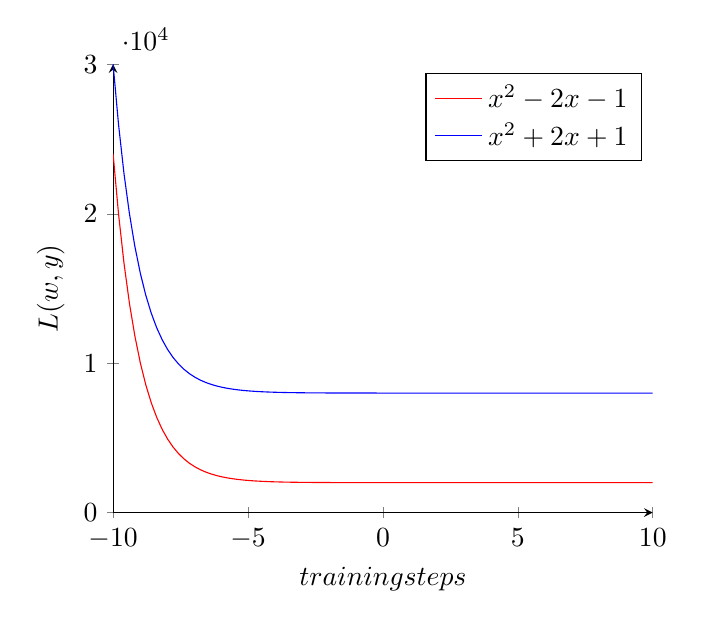
\begin{tikzpicture}
    \begin{axis}[
        axis lines = left,
        xlabel = $training steps$,
        ylabel = {$L(w,y)$},
        ymin=0,
    ]
    %Below the red parabola is defined
    \addplot [
        domain=-10:10, 
        samples=100, 
        color=red,
    ]
    {e^-x + 2000};
    \addlegendentry{$x^2 - 2x - 1$}
    %Here the blue parabloa is defined
    \addplot [
        domain=-10:10, 
        samples=100, 
        color=blue,
        ]
        {e^-x + 8000};
    \addlegendentry{$x^2 + 2x + 1$}
     
    \end{axis}
    \end{tikzpicture}